\section*{Exercice 160 -- Géométrie}
% Banque PT SIA 2013 CLever

\setcounter{exo}{0}
On s'intéresse à un véhicule triporteur permettant de s'incliner en virage.
\begin{center}
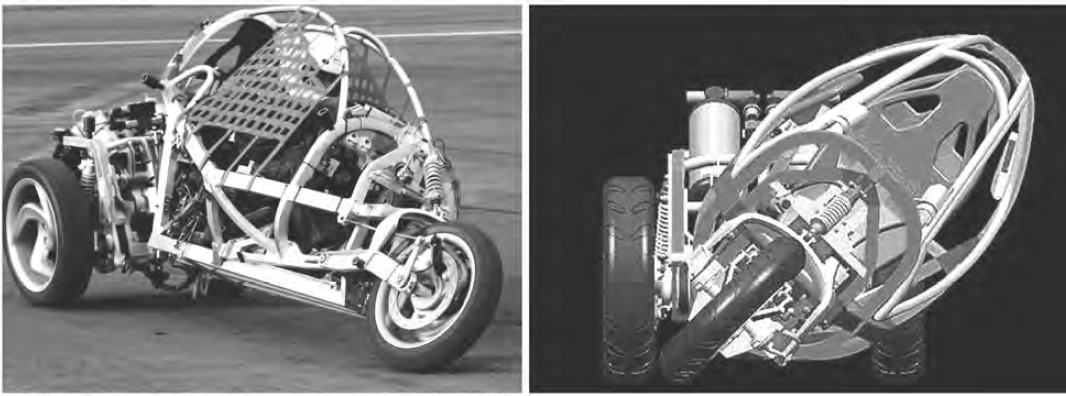
\includegraphics[width=\linewidth]{050_01}
\end{center}

On suppose que le mécanisme étudié admet  $\left(O,\vect{z_0},\vect{x_0} \right)$ comme plan d'étude. Le modèle cinématique adopté est précisé par le schéma cinématique de la figure suivante, sur laquelle sont aussi représentées les données géométriques et les paramètres de mouvements qui seront utilisés dans la question suivante afin de simplifier l'étude.


\begin{center}
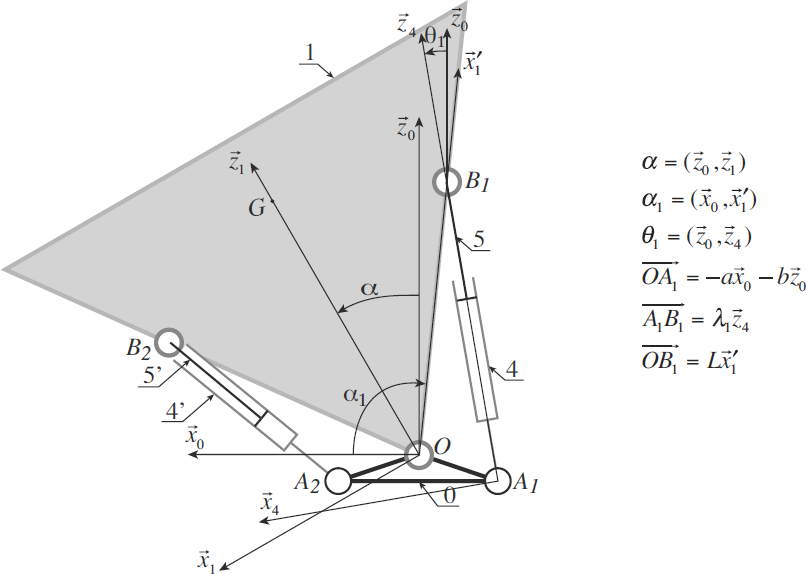
\includegraphics[width=\linewidth]{050_02}
\end{center}
 
\subparagraph{}
\textit{Déterminer 2 équations scalaires reliant $\alpha_1$ (on a $\alpha=\alpha_1-\alpha_{10}$, avec $\alpha_{10}$ valeur de $\alpha_{1}$ pour l'habitacle non-incliné), $\theta_1$ et $\lambda_1$ (les directions de projection seront judicieusement choisies). En éliminant le paramètre $\theta_1$, mettre la relation entre $\alpha_{1}$ et $\lambda_1$ sous la forme :
$\cos\left(\alpha_1+\psi\right)=\dfrac{A}{B}$ en précisant les expressions de $\psi$, $A$ et $B$ en fonction de $a$, $b$, $L$ et $\lambda_1$.}
\ifprof
\begin{corrige}

\end{corrige}
\else
\fi


Le tracé de cette relation est laborieux sans moyen numérique. Aussi, il vous est proposé de déterminer la position de
certains points de la courbe $\alpha\left( \lambda_1 \right)$ en prenant 2 positions d'inclinaison de l'habitacle entre 0 et
45\degres. On obtient ainsi 7 points pour la plage de variation de $\alpha$ (de $- 45\degres$ à $45\degres$). Pour cela,
on adopte le paramétrage 
de la figure suivante
en prenant comme origine des angles la position 
<< habitacle non-incliné >>.

\begin{center}
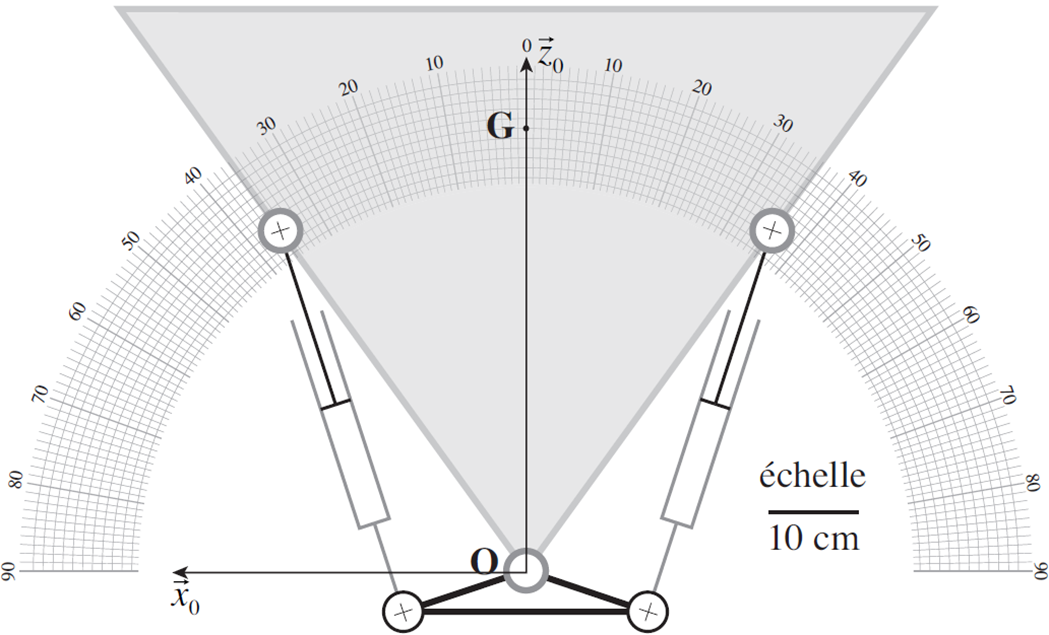
\includegraphics[width=\linewidth]{050_03}
\end{center}
 

\subparagraph{}
\textit{Représente les positions des points $B_1$ et $B_2$ pour les 2 positions angulaires choisies. Tracer l'évolution de $\alpha$ en fonction de $\lambda_1$ pour $\alpha$ compris entre $- 45\degres$ et $+ 45\degres$. Est-il possible de décrire cette courbe par une fonction linéaire en prenant comme origine les valeurs des paramètres pour la position <<~habitacle non-incliné~>> (on définit alors le paramètre $\lambda$ tel que : $\lambda = \lambda_1 - \lambda_{10}$) ? Si oui, donner une valeur approximative de sa pente, paramètre noté $R$ pour la suite.}
\ifprof
\begin{corrige}
\end{corrige}
\else
\fi
